%%%%%%%%%%%%%%%%%%%%%%%%%%%%%%%%%%%%%%%%
% BCS LaTeX template
% Version: 1.2
%%%%%%%%%%%%%%%%%%%%%%%%%%%%%%%%%%%%%%%%
\documentclass[a4paper, DIV=12, abstracton]{scrreprt}
\setcounter{secnumdepth}{3}


%%%%%%%%%%%%%%%%%%%%%%%%%%%%%%%%%%%%%%%%
% author and thesis details (please adjust accordingly)
%%%%%%%%%%%%%%%%%%%%%%%%%%%%%%%%%%%%%%%%
\newcommand{\name}{Gizem Ekinci} % <-- your name here
\title{Bayesian Inference of Information Transfer in Graph-Based Continuous-Time Multi-Agent Systems} % <-- thesis title here
\newcommand{\documenttype}{Master-Thesis} % <-- select type: "Master-Thesis", "Bachelor-Thesis", "Projektseminar", "Proseminar"
\newcommand{\major}{Elektro- und Informationstechnik} % <-- your study program
\newcommand{\supervisor}{Dominik Linzner} % <-- your supervisor here
\newcommand{\submission}{07.07.2020} % <-- your submission date here
%%%%%%%%%%%%%%%%%%%%%%%%%%%%%%%%%%%%%%%%

%%% load document settings %%%
%%%%%%%%%%%%%%%%%%%%%%%%%%%%%%%%%%%%%%%%
% packages
%%%%%%%%%%%%%%%%%%%%%%%%%%%%%%%%%%%%%%%%

%%% math %%%
\usepackage{amsmath}
\usepackage{amssymb}
\usepackage{mathtools}
\usepackage{unicode-math}

%%% fonts %%%
\usepackage{lmodern}

%%% graphics %%%
\usepackage{tikz, wrapfig}
\graphicspath{{figures/}}
\usepackage{subcaption}
\usepackage{float}
\usepackage{graphicx}
\usetikzlibrary{positioning}
\usetikzlibrary{arrows}

%%% bibliography %%%
\bibliographystyle{plain}
\usepackage{etoolbox}
\AtBeginEnvironment{thebibliography}{\interlinepenalty=10000}

%%% misc %%%
\usepackage{blindtext}

%%% algorithms %%%
\usepackage{algorithmic}
\usepackage[ruled, lined, longend]{algorithm2e}

%%% referencing %%%
\usepackage[bookmarks, bookmarksdepth=chapter, hidelinks]{hyperref}
\usepackage[capitalise, noabbrev]{cleveref}
\newcommand{\crefrangeconjunction}{-}
\usepackage{xr}


%%%%%%%%%%%%%%%%%%%%%%%%%%%%%%%%%%%%%%%%
% document settings
%%%%%%%%%%%%%%%%%%%%%%%%%%%%%%%%%%%%%%%%

%%% title page %%%
\author{}
\date{}
\titlehead{
	\centering
	
\includegraphics[width=10cm]{tud_logo.pdf} \\
	\large\sffamily
	Fachbereich Elektrotechnik und Informationstechnik \\
	Bioinspired Communication Systems
	\vspace{10ex}
} 
\subtitle{
	\vspace{2ex}
	\documenttype\\
	\normalfont \sffamily 
	\major \\
	\vspace{4ex}
	Eingereicht von\\
	\vspace{2ex}
	{\Large \name}\\
	\vspace{2ex}
	am\\
	\submission\\
	\vspace{4ex}
	\parbox{0cm}{%
	\begin{tabbing}
	1.~Gutachten: \= Prof.~Dr.~techn.~Heinz~Koeppl \\
	2.~Gutachten: \>\supervisora \\
	3.~Gutachten: \>\supervisorb
	\end{tabbing}}
}

%%% paragraph settings %%%
\parindent0ex
\parskip\baselineskip



%%%%%%%%%%%%%%%%%%%%%%%%%%%%%%%%%%%%%%%%
% commands
%%%%%%%%%%%%%%%%%%%%%%%%%%%%%%%%%%%%%%%%

%%% probability %%%
\newcommand{\given}{\,|\,}
\newcommand{\p}{p}

\DeclareRobustCommand{\rchi}{{\mathpalette\irchi\relax}}
\newcommand{\irchi}[2]{\raisebox{\depth}{$#1\chi$}}
\DeclareMathOperator*{\argmax}{arg\,max}
\DeclareMathOperator*{\argmin}{arg\,min}

\RedeclareSectionCommands[
	beforeskip=-3.25ex plus -1ex minus -0.2ex,
	runin=false,
	afterskip=2sp
]{paragraph,subparagraph}

\begin{document}
	\maketitle
	\pagestyle{empty}\ \newpage

\paragraph*{Erkl\"arung zur Abschlussarbeit gem\"a\ss~$\boldsymbol{\S}$22 Abs.~7 und $\boldsymbol{\S}$23 Abs.~7 APB TU Darmstadt}\ \\[\baselineskip]
Hiermit versichere ich, \name, die vorliegende Arbeit gem\"a\ss~\S 22 Abs.~7 APB der TU Darmstadt ohne Hilfe Dritter und nur mit den angegebenen Quellen und Hilfsmitteln angefertigt zu haben. Alle Stellen, die Quellen entnommen wurden, sind als solche kenntlich gemacht worden. Diese Arbeit hat in gleicher oder \"ahnlicher Form noch keiner Pr\"ufungsbeh\"orde vorgelegen. Mir ist bekannt, dass im Falle eines Plagiats (\S38 Abs.2 APB) ein T\"auschungsversuch vorliegt, der dazu f\"uhrt, dass die Arbeit mit 5,0 bewertet und damit ein Pr\"ufungsversuch verbraucht wird. Abschlussarbeiten d\"urfen nur einmal wiederholt werden. Bei der abgegebenen Arbeit stimmen die schriftliche und die zur Archivierung eingereichte elektronische Fassung gem\"a\ss\ \S 23 Abs.~7 APB \"uberein.\\

English translation for information purposes only:\\[\baselineskip]
Thesis statement pursuant to \S22 paragraph 7 and \S23 paragraph 7 of APB TU Darmstadt:\\
I herewith formally declare that I, \name, have written the submitted thesis independently pursuant to \S22 paragraph 7 of APB TU Darmstadt. I did not use any outside support except for the quoted literature and other sources mentioned in the paper. I clearly marked and separately listed all of the literature and all of the other sources which I employed when producing this academic work, either literally or in content. This thesis has not been handed in or published before in the same or similar form.
I am aware, that in case of an attempt at deception based on plagiarism (§38 Abs. 2 APB), the thesis would be graded with 5,0 and counted as one failed examination attempt. The thesis may only be repeated once. In the submitted thesis the written copies and the electronic version for archiving are pursuant to § 23 paragraph 7 of APB identical in content.\\


Darmstadt, den \submission\\

\rule{6cm}{0.7pt}\\
(\name)

	\newpage \
\newpage

\begin{abstract}
	Multi-agent systems in nature, such as a population of cells, cooperate through information sharing. This information can be incomplete and noisy. Inspired by such systems, we consider communication between three individuals, which are evolving continuously in time. Two of them act independently, and emit messages containing information about their states, while the third one receives a translation of these messages. Based on these translated observations, the agent node forms its belief over the state of other nodes. We modelled this system combining continuous-time Bayesian network (CTBN) and partially observable Markov decision (POMDP) process frameworks. The nodes evolve continuously in time as components of a CTBN. Given that the true messages are unavailable to the agent, the interaction between the nodes is modelled as POMDP. The exact update of the belief state is computed by filtering, and these results are used as a baseline. The approximation of the belief state is obtained using marginalized particle filtering. This work aims to infer the language model which leads to the translations.\\
	%The belief state is updated utilising two methods. The first one is exact update, discussed in \cref{par:bs_exact}, and assumes that the transition intensities of the parents $ \textbf{Q}_1 $ and $ \textbf{Q}_2 $ are available both for the agent and for the classifier. However, due to the fact that this would not present a realistic system, particle filtering with marginalized CTBN is introduced for as state estimator. Here, both the agent and the classifier was able to perform the belief state update, given Gamma-priors of $ \textbf{Q}_1 $ and $ \textbf{Q}_2 $.\\
\end{abstract}

\newpage \
\newpage
	
	\tableofcontents
	\thispagestyle{empty}
	\newpage
	\setcounter{page}{1}

	\chapter{Introduction}

\blindtext

\section{Problem Statement}

\blindtext

\section{Related Work}

\blindtext

\section{Contributions}

\blindtext
	\chapter{Theoretical Background}
\blindtext

\section{Continuous Time Bayesian Networks}
The entire communication is defined in the framework of continuous-time Bayesian network (CTBN).
\subsection{Time-homogenous continuous-time Markov Processes}
The messages that are emitted by the cells are modelled as independent time-homogeneous continuous-time Markov processes (CTMP). These processes are defined by transition intensity matrices $ Q_{X} $ and $ Q_{Y} $, whose intensities does not depend on time. In this matrix, the intensity $ q_{i} $ represents the instantaneous probability of leaving state i and $ q_{i,j} $ represents the instantaneous probability of switching from state $ i $ to $ j $. %TODO give a Q matrix and explain further

Infinitesimal transition probabilities in terms of the entries of transition matrices $ q_{ij} $ can be written as \cite{Cohn2010a}:
\begin{equation}
p_{i,j}(h)=\delta_{ij}+q_{i,j} h+o(h)
\end{equation}
where $ p_{i, j}(t) \equiv Pr(X^{(t+s)}=j\mid X^{(s)}=i) $ are Markov transition functions and o(.) is a function decaying to zero faster than its argument.

The \textit{forward} or \textit{master equation} is then derived as follows:

\begin{equation}
p_{j}(t)=\sum_{\forall i} p_{i, j}(h) p_{i}(t-h)
\end{equation}

\begin{equation}
\begin{split}
\lim_{h\rightarrow 0} p_{j}(t) & = \lim_{h\rightarrow 0} \sum_{\forall i} \left[ \delta_{ij}+q_{i,j} h+o(h)\right]  p_{i}(t-h) \\ & = \lim_{h\rightarrow 0} p_{j}(t-h) + \lim_{h\rightarrow 0} h \sum_{\forall i} q_{i,j} p_{i}(t-h)
\end{split}
\end{equation}

\begin{equation}
\lim_{h\rightarrow 0} \frac{p_{j}(t) - p_{j}(t-h)}{h} = \lim_{h\rightarrow 0} \sum_{\forall i} q_{i,j} p_{i}(t-h)
\end{equation}

\begin{equation}
\begin{split}
\frac{d}{dt} p_{j}(t) & = \sum_{\forall i} q_{i,j} p_{i}(t) \\ & = \sum_{\forall i \neq j}\left[  q_{i,j} p_{i}(t) - q_{j,i} p_{j}(t) \right]
\end{split}
\label{eq:ME}
\end{equation}
Eq.\ref{eq:ME} can be written in matrix form:
\begin{equation}
\frac{d}{dt} p = p\textbf{Q}
\end{equation}
The solution to ODE, the time-dependent probability distribution $ p(t) $ is, 
\begin{equation}
p(t)=p(0) \exp (t\textbf{Q})
\end{equation}
with initial distribution $ p(0) $.

The amount of time staying in a state i is exponentially distributed with parameter $ q_{i} $. The probability density function f for staying in the state $ i $:
\begin{equation}
f(t)=q_{i} \exp \left(-q_{i} t\right), t\geq 0
\label{eq:f(t)_homo}
\end{equation}
\subsubsection{The Likelihood Function}
To write down the likelihood of a trajectory sampled from a homogenous CTMC $ X $, first let us consider one transition $ d = <i,j,t> $, where transition happens after time t from state i to j. The likelihood of this transition is:
\begin{equation}
L_{X}(d \mid \textbf{Q})=\left(q_{i} \exp \left(-q_{i} t\right)\right)\left(\frac{q_{i,j}}{q_{i}}\right)
\end{equation}
We define sufficient statistics over a dataset $ D $ as $ T[i] $, total amount of time spent in state i, $ M[i,j] $ total number of transitions from state i to j, we can write down the likelihood of a trajectory $  X^{\left[0,T\right] } $,
\begin{equation}
\begin{split}
L_{X}(\textbf{Q} : D) &=  \prod_{d \in D} L(d \mid \textbf{Q}) \\&=\left(\prod_{\forall i} q_{i}^{M[i]} \exp \left(-q_{i} T[i]\right)\right)\left(\prod_{\forall i} \prod_{\forall j \neq i} \left(\frac{q_{i,j}}{q_{i}}\right)^{M\left[i, j\right]}\right)
\label{eq:lh_traj_homo}
\end{split}
\end{equation}
with $ M[i] = \sum_{\forall j} M[i, j] $.

\subsection{Time-inhomogeneous continuous-time Markov Processes}
In an conventional CTBN, while every node is a Markov process itself, the leaf nodes are \textit{conditional} Markov processes, a type of inhomogeneous Markov process, where the intensities change over time, but not as a function of time rather as a function of parent states. \cite{Nodelman1995} %TODO explain time-dependence in the problem
 
For inhomogeneous Markov processes, Eq.\ref{eq:f(t)_homo} becomes:
\begin{equation}
f(t) = q_{i}(t) \exp \left(-\int_{0}^{t} q_{i}(u) d u\right)
\end{equation}
\subsubsection{The Likelihood Function}
Let X be an inhomogeneous Markov process, and $  X^{\left[0,T\right] } $ is a trajectory sampled from this process. We define $ m $ number of transitions, with $ 0 = t_{0} < t_{1} < ... < t_{m} $ are the times where transition occurred, and $ x_{0}, x_{1},..., x_{m} $ are the observed states. The likelihood of trajectory  $  X^{\left[0,T\right] } $ is  as follows: 
\begin{equation}
L(\textbf{Q}_{X} \colon  X^{\left[0,T\right]} ) = \prod_{k=1}^{m} \left[ q_{x_{k-1}} (t_{k}) \exp \left(-\int_{t_{k-1}}^{t_{k}} q_{x_{k-1}}(u) d u\right) \frac{q_{x_{k-1}, x_{k}} (t_{k})}{q_{x_{k-1}}(t_{k})}\right] 
\label{eq:lh_traj_inhomo}
\end{equation}

We can formulate our graphical model as $ S = [X, Y, Z] $, where $ Par(Z) = {X,Y} $ and $ Par(X) = Par(Y) =\emptyset $. We can then write the conditional probability:
\begin{equation}
\begin{split}
P\left(S^{\left(t+h\right)}=s' | S^{\left(t\right)}=s\right) = & P\left(X^{\left( t+h\right) }=x' | X^{\left(t\right)}=x, Par(X)^{\left(t\right)}={y,z}\right) \\&  P\left(Y^{\left( t+h\right) }=y' | Y^{\left(t\right)}=y\right) P\left(Z^{\left( t+h\right) }=z' | ^{\left(t\right)}=z\right)
\end{split} 
\end{equation}

\section{Partially observable Markov Decision Processes}
In our problem, cell Z does not have a direct access to its parents' states, rather it observes a summary of them. This is different than observing the states through noisy binary channels, and presents a POMDP problem. Even though it is assumed that the policy of Z is optimal given the true states of parents, the problem of inferring the observational model remains unsolved and to be addressed.

In a conventional POMDP, given the \textit{transition function}, $ T(s, a, s^{\prime})$  and \textit{observation function}, $ O(s^{\prime}, a, o) $, the belief state update is computed as follows \cite{Kaelbling2011} \footnote{Since for now, we assume there is no affect of Z's action on the observation or transition function, $ a $ is omitted from the equation.}:
\begin{equation}
\begin{aligned}
b^{\prime}\left(s^{\prime}\right) &=\operatorname{Pr}\left(s^{\prime} | o, a, b\right) =\operatorname{Pr}\left(s^{\prime} | o, b\right) \\
&=\frac{\operatorname{Pr}\left(o | s^{\prime}, b\right) \operatorname{Pr}\left(s^{\prime} | b\right)}{\operatorname{Pr}(o | b)} \\
&=\frac{\operatorname{Pr}\left(o | s^{\prime}\right) \sum_{s \in \mathcal{S}} \operatorname{Pr}\left(s^{\prime} | b, s\right) \operatorname{Pr}(s | b)}{\operatorname{Pr}(o | b)} \\
&=\frac{O\left(s^{\prime}, o\right) \sum_{s \in \mathcal{S}} T\left(s, s^{\prime}\right) b(s)}{\operatorname{Pr}(o | b)}
\end{aligned}
\label{eq:b}
\end{equation}

In Eq.\ref{eq:b}, the transition function is time-independent. However, in our setting, the parent nodes X and Y are modelled as CTMCs with time-dependent transition matrices. To derive \textit{continuous-time belief state}, $ b(t) $, first we need to get the joint transition matrix of X and Y, two independent processes. This operation called \textit{amalgamation} is described in detail by Nodelman \textit{et al} \cite{Nodelman1995}. Let us denote this matrix by $ Q_{XY} $. 
Now we can derive the belief state as follows: 

\begin{equation}
b_{s^{\prime}}(t) =\frac{\operatorname{Pr}\left(o |s^{\prime}\right) \sum_{s \in \mathcal{S}} \operatorname{Pr}\left(S(t)=s^{\prime} | S(t-h)=s\right) b_{s}(t-h)}{\operatorname{Pr}(o | b)}
\end{equation}\\
\begin{equation}
\begin{aligned}
\lim_{h\rightarrow 0} b_{s^{\prime}}(t) &= C \lim_{h\rightarrow 0}\left[  \sum_{s \in \mathcal{S}} p_{s, s^{\prime}}(t) b_{s}(t-h)\right]\\
&= C \lim_{h\rightarrow 0}\left[  \sum_{s \in \mathcal{S}} \left[ \delta_{ss^{\prime}}+q_{s,s^{\prime}} h+o(h)\right]  b_{s}(t-h)\right]\\
&= C \lim_{h\rightarrow 0}\left[ b_{s^{\prime}}(t-h) + \sum_{s \in \mathcal{S}} q_{s,s^{\prime}} h  b_{s}(t-h)\right]
\end{aligned}
\end{equation}
Due to the scaling factor $ C =\frac{\operatorname{Pr}\left(o |s^{\prime}\right)}{\operatorname{Pr}(o | b)} $, cannot derive $ \frac{d}{dt} b = \textbf{Q}b$, .\\
However, we can use the conditional distribution of Markov processes as the transition function $ T(s'|s) $ to derive the continuous-time belief state. The conditional distribution over the value of X, a homogenous Markov process, at time t given its value at an earlier time s can be written as 
\begin{equation}
\operatorname{Pr}\left(X(t) \mid X(s)\right) = \exp(\textbf{Q}(t-s))
\end{equation}
Then the continuous-time belief state becomes:
\begin{equation}
b_{s^{\prime}}(t) =\frac{\operatorname{Pr}\left(o |s^{\prime}\right) \sum_{s \in \mathcal{S}}\left[ \exp(\textbf{Q}(h))\right]_{s,s'}  b_{s}(t-h)}{\operatorname{Pr}(o | b)}
\end{equation}

	\chapter{Methodology}
\blindtext

\section{Data Generation - Simulation}
\section{Inference of Deterministic Observation Model}
Our dataset contains a number of trajectories from all the nodes involved in the communication. $ \textbf{D} = \left\lbrace D_{1},..., D_{N}\right\rbrace $. Every trajectory comprises of state transitions in time interval $  [0, T] $, and the times of these transitions.

	\chapter{Results}


\section{Simulation}
\begin{figure}[htb]
	\begin{center}
		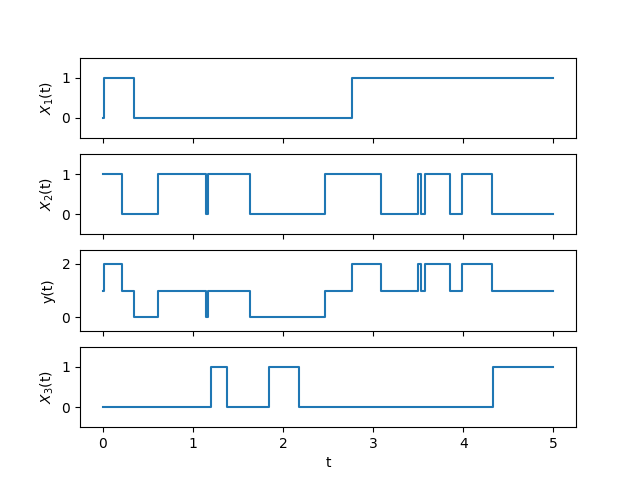
\includegraphics[width=.50\textwidth]{figures/traj}
		\caption{Sampled trajectories}
		\label{fig:traj}
	\end{center}
\end{figure}
\begin{figure}[htb]
	\begin{center}
		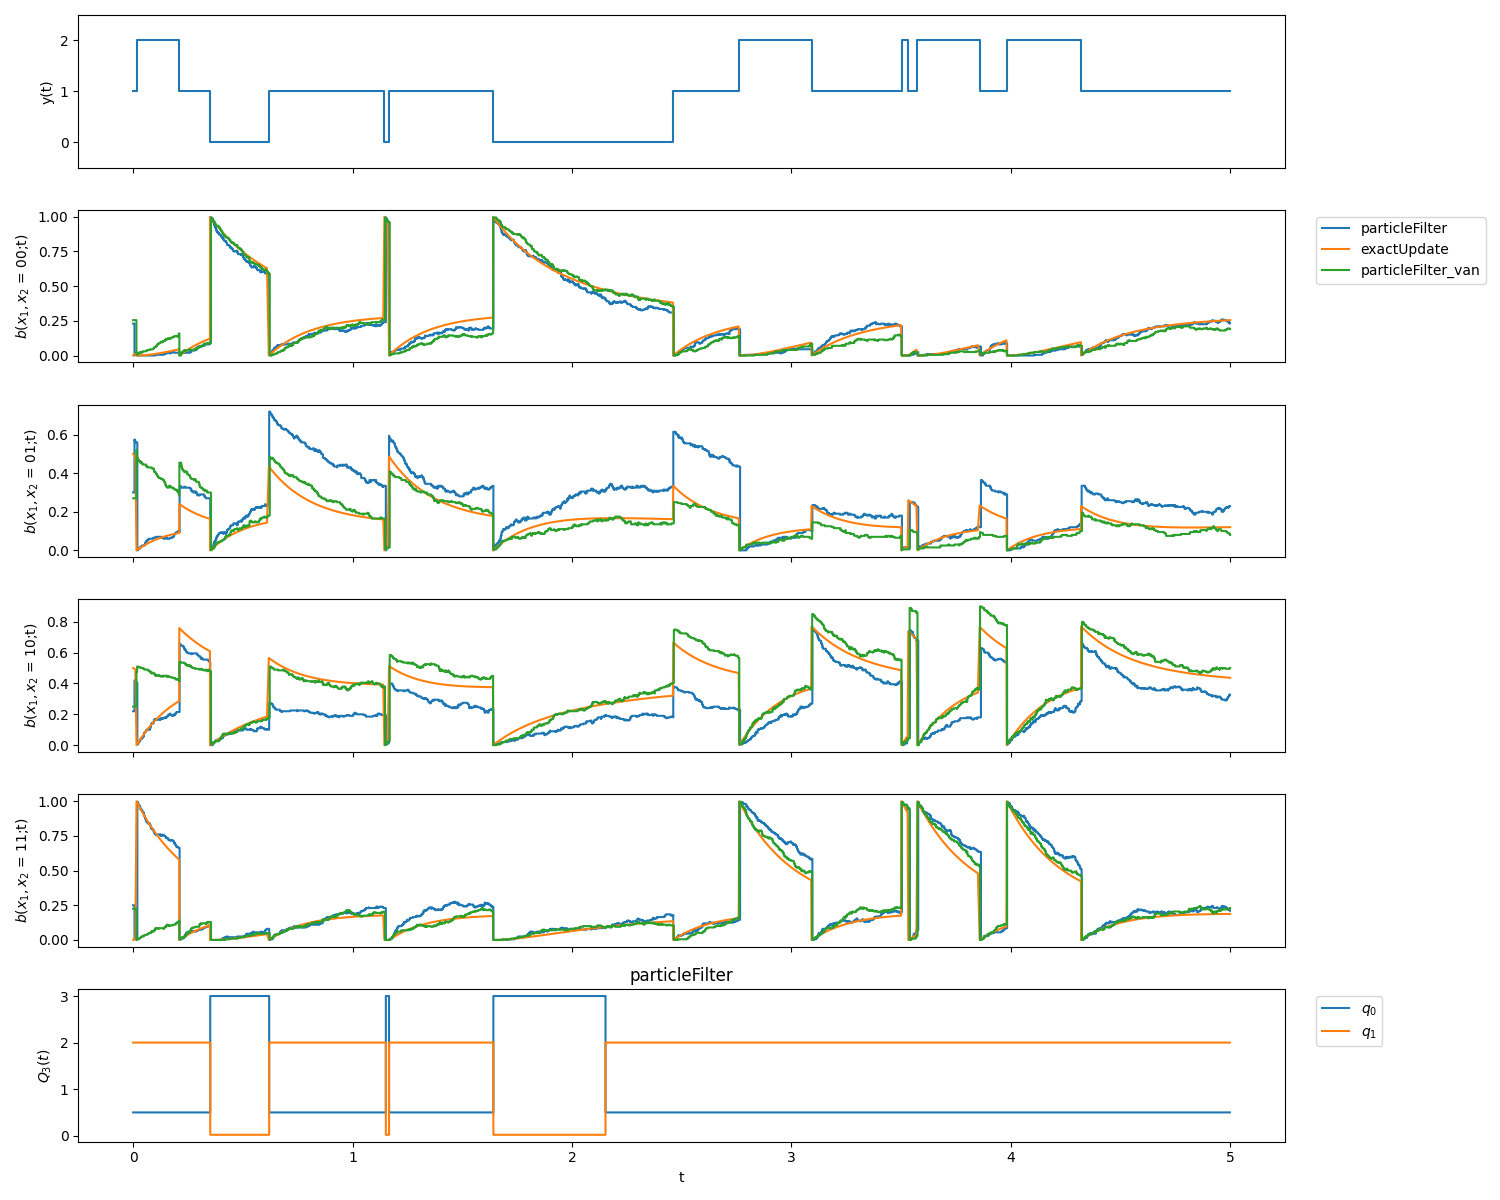
\includegraphics[width=.50\textwidth]{figures/b_q_traj}
		\caption{Belief state and $ Q_3 $ trajectories}
		\label{fig:b_q_traj}
	\end{center}
\end{figure}

\section{Results}
\subsection{Maximum Likelihood Estimation}
$\psi_{true} =
\begin{bmatrix} \vspace{-2pt}
	1 & 0 & 0 \\  \vspace{-2pt}
	0 & 1 & 0 \\  \vspace{-2pt}
	0 & 1 & 0 \\  \vspace{-1pt}
	0 & 0 & 1
\end{bmatrix}$
$\psi_{0} =
\begin{bmatrix} \vspace{-2pt}
1 & 0 & 0 \\  \vspace{-2pt}
0 & 1 & 0 \\  \vspace{-2pt}
0 & 1 & 0 \\  \vspace{-1pt}
0 & 0 & 1
\end{bmatrix}, 
\psi_{1} =
\begin{bmatrix} \vspace{-2pt}
0 & 0 & 1 \\  \vspace{-2pt}
0 & 1 & 0 \\  \vspace{-2pt}
1 & 0 & 0 \\  \vspace{-1pt}
0 & 0 & 1 
\end{bmatrix},
\psi_{2} =
\begin{bmatrix} \vspace{-2pt}
0 & 0 & 1 \\  \vspace{-2pt}
1 & 0 & 0 \\  \vspace{-2pt}
0 & 0 & 1 \\  \vspace{-1pt}
0 & 1 & 0  
\end{bmatrix}$
\begin{figure}[htb]
	\begin{subfigure}{.5\textwidth}
		\centering
		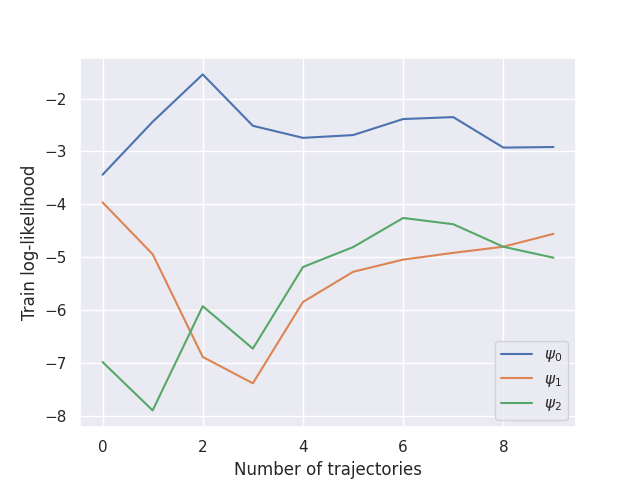
\includegraphics[width=1\linewidth]{figures/llh_[1.0, 0.0, 0.0]}
		\caption{}
		\label{fig:sfig1}
	\end{subfigure}%
	\begin{subfigure}{.5\textwidth}
		\centering
		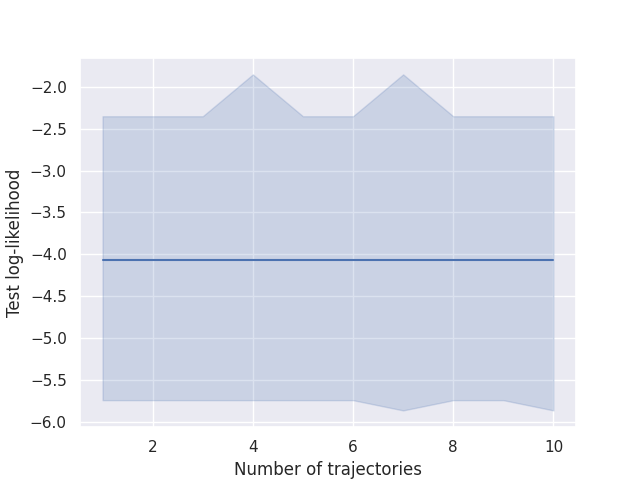
\includegraphics[width=1\linewidth]{figures/test_likelihood_particleFilter_[1.0, 0.0, 0.0]}
		\caption{}
		\label{fig:sfig2}
	\end{subfigure}
	\caption{plots of....}
	\label{fig:fig}
\end{figure}\\
$\psi_{true} =
\begin{bmatrix} \vspace{-2pt}
0.98 & 0.01 & 0.01 \\  \vspace{-2pt}
0.01 & 0.98 & 0.01 \\  \vspace{-2pt}
0.01 & 0.98 & 0.01 \\  \vspace{-1pt}
0.01 & 0.01 & 0.98
\end{bmatrix}$
$\psi_{0} =
\begin{bmatrix} \vspace{-2pt}
1 & 0 & 0 \\  \vspace{-2pt}
0 & 1 & 0 \\  \vspace{-2pt}
0 & 1 & 0 \\  \vspace{-1pt}
0 & 0 & 1
\end{bmatrix}, 
\psi_{1} =
\begin{bmatrix} \vspace{-2pt}
0 & 0 & 1 \\  \vspace{-2pt}
0 & 1 & 0 \\  \vspace{-2pt}
1 & 0 & 0 \\  \vspace{-1pt}
0 & 0 & 1 
\end{bmatrix},
\psi_{2} =
\begin{bmatrix} \vspace{-2pt}
0 & 0 & 1 \\  \vspace{-2pt}
1 & 0 & 0 \\  \vspace{-2pt}
0 & 0 & 1 \\  \vspace{-1pt}
0 & 1 & 0  
\end{bmatrix}$
\begin{figure}[htb]
	\begin{subfigure}{.5\textwidth}
		\centering
		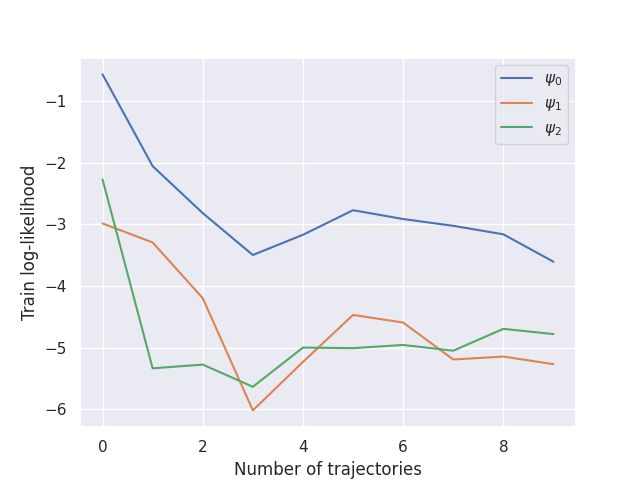
\includegraphics[width=1\linewidth]{figures/llh_[0.98, 0.01, 0.01]}
		\caption{}
		\label{fig:sfig1}
	\end{subfigure}%
	\begin{subfigure}{.5\textwidth}
		\centering
		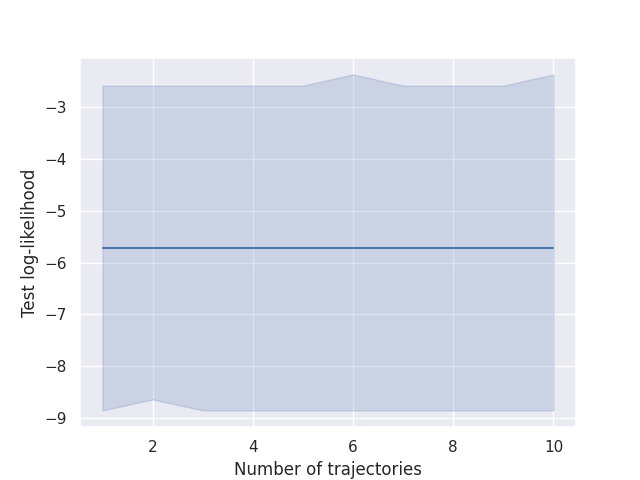
\includegraphics[width=1\linewidth]{figures/test_likelihood_particleFilter_[0.98, 0.01, 0.01]}
		\caption{}
		\label{fig:sfig2}
	\end{subfigure}
	\caption{plots of....}
	\label{fig:fig}
\end{figure}\\
$\psi_{true} =
\begin{bmatrix} \vspace{-2pt}
0.95 & 0.025 & 0.025 \\  \vspace{-2pt}
0.025 & 0.95 & 0.025 \\  \vspace{-2pt}
0.025 & 0.95 & 0.025 \\  \vspace{-1pt}
0.025 & 0.025 & 0.95
\end{bmatrix}$
$\psi_{0} =
\begin{bmatrix} \vspace{-2pt}
1 & 0 & 0 \\  \vspace{-2pt}
0 & 1 & 0 \\  \vspace{-2pt}
0 & 1 & 0 \\  \vspace{-1pt}
0 & 0 & 1
\end{bmatrix}, 
\psi_{1} =
\begin{bmatrix} \vspace{-2pt}
0 & 0 & 1 \\  \vspace{-2pt}
0 & 1 & 0 \\  \vspace{-2pt}
1 & 0 & 0 \\  \vspace{-1pt}
0 & 0 & 1 
\end{bmatrix},
\psi_{2} =
\begin{bmatrix} \vspace{-2pt}
0 & 0 & 1 \\  \vspace{-2pt}
1 & 0 & 0 \\  \vspace{-2pt}
0 & 0 & 1 \\  \vspace{-1pt}
0 & 1 & 0  
\end{bmatrix}$
\begin{figure}[htb]
	\begin{subfigure}{.5\textwidth}
		\centering
		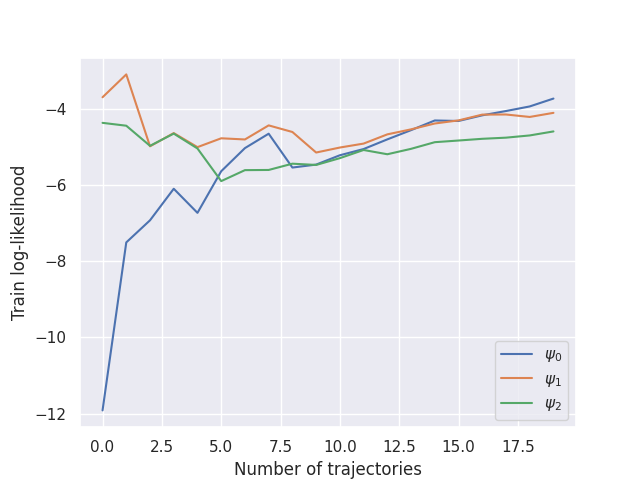
\includegraphics[width=1\linewidth]{figures/llh_particleFilter_[0.95, 0.025, 0.025]}
		\caption{}
		\label{fig:sfig1}
	\end{subfigure}%
	\begin{subfigure}{.5\textwidth}
		\centering
		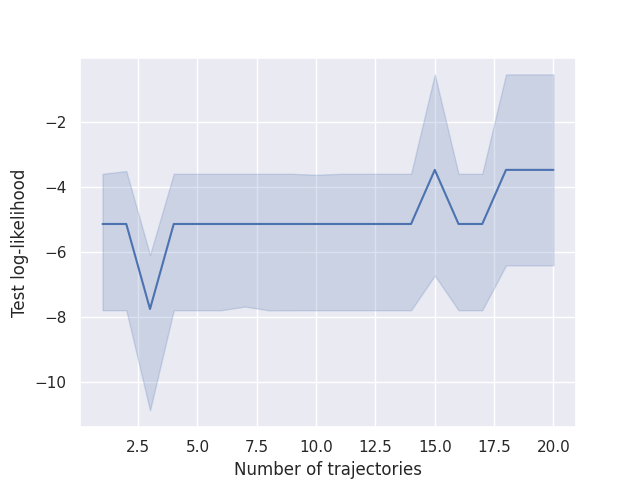
\includegraphics[width=1\linewidth]{figures/test_likelihood_particleFilter_[0.95, 0.025, 0.025]}
		\caption{}
		\label{fig:sfig2}
	\end{subfigure}
	\caption{plots of....}
	\label{fig:fig}
\end{figure}\\
$\psi_{true} =
\begin{bmatrix} \vspace{-2pt}
0.9 & 0.05 & 0.05 \\  \vspace{-2pt}
0.05 & 0.9 & 0.05 \\  \vspace{-2pt}
0.05 & 0.9 & 0.05 \\  \vspace{-1pt}
0.05 & 0.05 & 0.9
\end{bmatrix}$
$\psi_{0} =
\begin{bmatrix} \vspace{-2pt}
1 & 0 & 0 \\  \vspace{-2pt}
0 & 1 & 0 \\  \vspace{-2pt}
0 & 1 & 0 \\  \vspace{-1pt}
0 & 0 & 1
\end{bmatrix}, 
\psi_{1} =
\begin{bmatrix} \vspace{-2pt}
0 & 0 & 1 \\  \vspace{-2pt}
0 & 1 & 0 \\  \vspace{-2pt}
1 & 0 & 0 \\  \vspace{-1pt}
0 & 0 & 1 
\end{bmatrix},
\psi_{2} =
\begin{bmatrix} \vspace{-2pt}
0 & 0 & 1 \\  \vspace{-2pt}
1 & 0 & 0 \\  \vspace{-2pt}
0 & 0 & 1 \\  \vspace{-1pt}
0 & 1 & 0  
\end{bmatrix}$
\begin{figure}[htb]
	\begin{subfigure}{.5\textwidth}
		\centering
		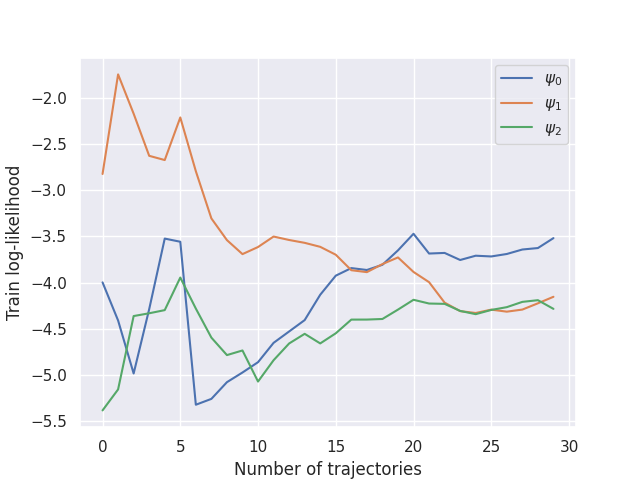
\includegraphics[width=1\linewidth]{figures/llh_particleFilter_van}
		\caption{}
		\label{fig:sfig1}
	\end{subfigure}%
	\begin{subfigure}{.5\textwidth}
		\centering
		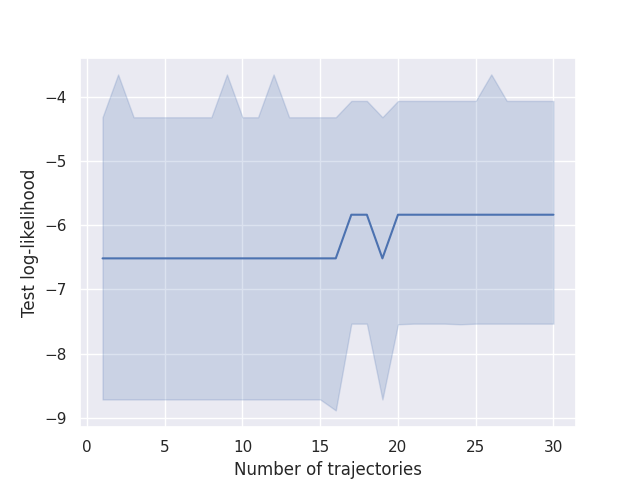
\includegraphics[width=1\linewidth]{figures/test_likelihood_particleFilter_van}
		\caption{}
		\label{fig:sfig2}
	\end{subfigure}
	\caption{plots of....}
	\label{fig:fig}
\end{figure}

\subsection{Maximum Likelihood Classification}
\begin{figure}[htb]
	\begin{subfigure}{.33\textwidth}
		\centering
		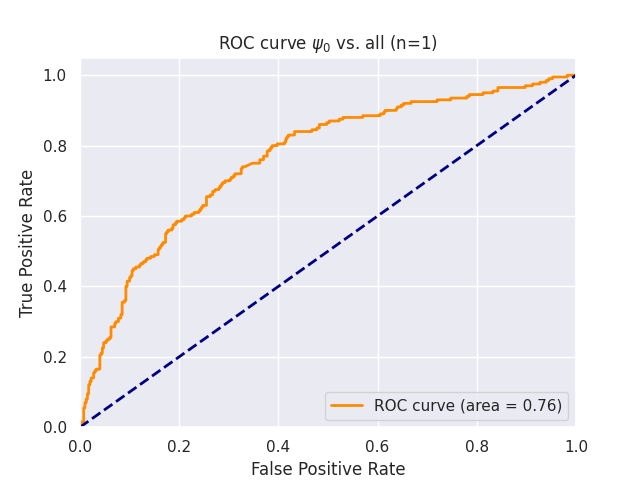
\includegraphics[width=1\linewidth]{figures/AUROC_600samples_class0_llh_n1}
		\caption{}
		\label{fig:sfig1}
	\end{subfigure}%
	\begin{subfigure}{.33\textwidth}
		\centering
		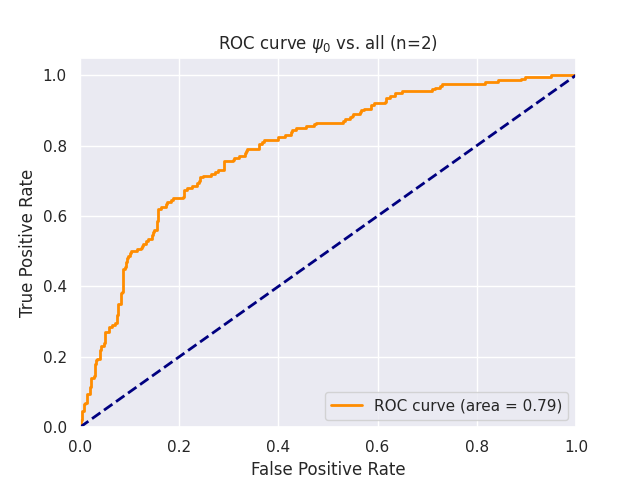
\includegraphics[width=1\linewidth]{figures/AUROC_600samples_class0_llh_n2}
		\caption{}
		\label{fig:sfig2}
	\end{subfigure}
	\begin{subfigure}{.33\textwidth}
		\centering
		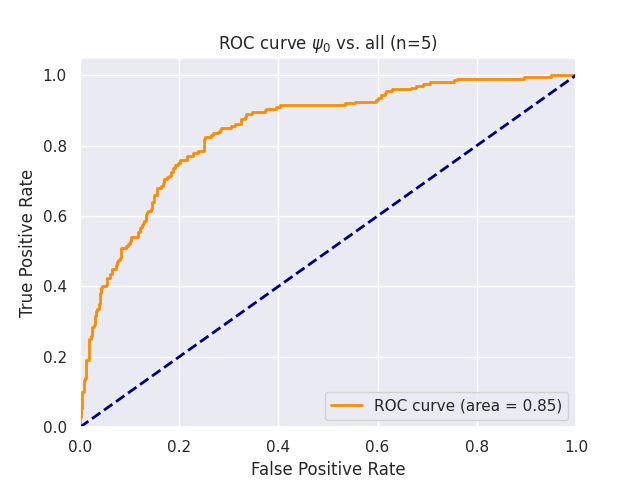
\includegraphics[width=1\linewidth]{figures/AUROC_600samples_class0_llh_n5}
		\caption{}
		\label{fig:sfig2}
	\end{subfigure}\\
	\begin{subfigure}{.33\textwidth}
		\centering
		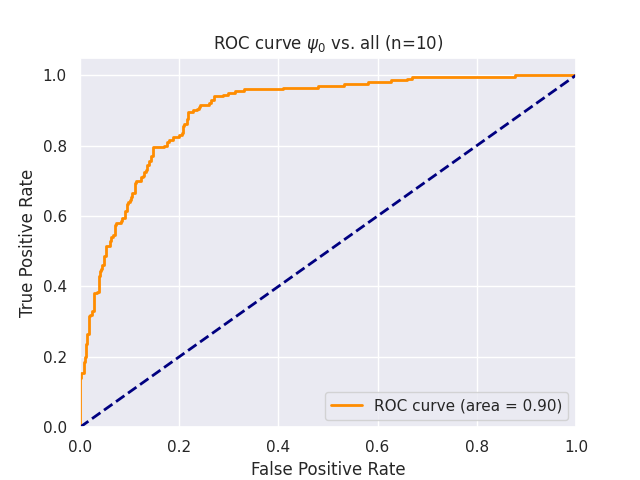
\includegraphics[width=1\linewidth]{figures/AUROC_600samples_class0_llh_n10}
		\caption{}
		\label{fig:sfig1}
	\end{subfigure}%
	\begin{subfigure}{.33\textwidth}
		\centering
		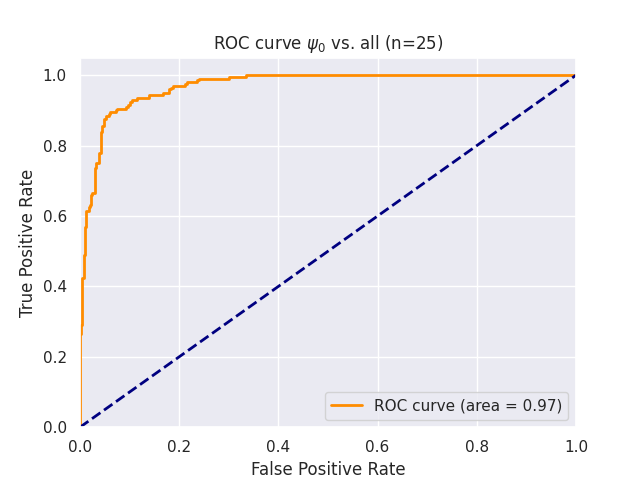
\includegraphics[width=1\linewidth]{figures/AUROC_600samples_class0_llh_n25}
		\caption{}
		\label{fig:sfig2}
	\end{subfigure}
	\begin{subfigure}{.33\textwidth}
		\centering
		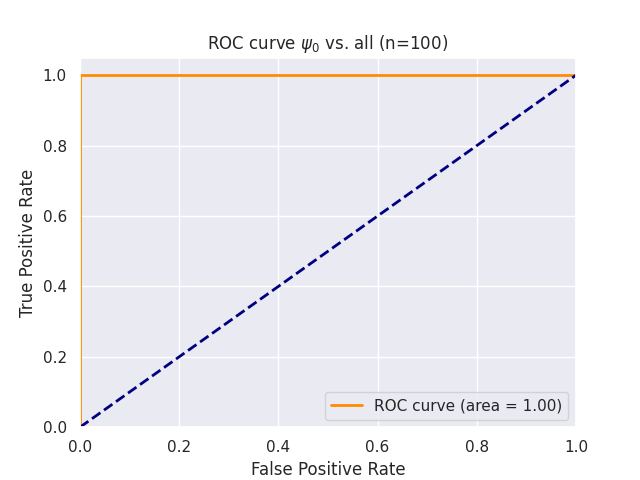
\includegraphics[width=1\linewidth]{figures/AUROC_600samples_class0_llh_n100}
		\caption{}
		\label{fig:sfig2}
	\end{subfigure}\\
	\caption{plots of....}
	\label{fig:fig}
\end{figure}
\begin{figure}[htb]
	\begin{center}
		\includegraphics[width=.9\textwidth]{figures/all_particlefilter}
		\caption{plot of...}
		\label{fig:traj}
	\end{center}
\end{figure}

	\chapter{Conclusion}
\blindtext

\section{Discussion}
\Blindtext
\Blindtext

\section{Future Work}
\Blindtext
	\bibliography{../bibtex/_master_thesis}
\end{document}